\section{Business Process Modeling Notation}
V roku 2004 bol Business Process Management Initiative (BPMI) vydan� �tandard BPMN 1.0. Cie�om tohoto �tandardu je poskytn�� �ahko pochopite�n� not�ciu pre v�etk�ch u��vate�ov podie�aj�cich sa na tvoren�, implement�cii, spravovan� a monitorovan� firemn�ch procesov. S��as�ou BPMN je aj intern� model, ktor� umo��uje prevod na spustite�n� BPEL4WS k�d. Vyp��a sa t�m medzera medzi firemn�m procesn�m n�vrhom a implement�ciou. \\
BPMN definuje Business Process Diagram (BPD), ktor� graficky zn�zor�uje postupnosti firemn�ch procesov. Objekty zachyten� v grafe reprezentuj� aktivity a orientovan� hrany nazna�uj� poradie ich vykonania. 

\subsection{Rozdelenie objektov v BPMN}

\subsection{Flow Objects }
\begin{center}
\includegraphics{pic/activity.png}\end{center}
\begin{center}
\includegraphics{pic/event.png}\end{center}
\begin{center}
\includegraphics{pic/gateway.png}\end{center}

\subsubsection{Artifacts}
\begin{center}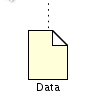
\includegraphics{pic/data.png}\end{center}
\begin{center}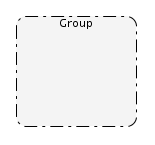
\includegraphics{pic/group.png}\end{center}
\begin{center}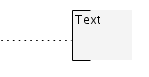
\includegraphics{pic/annotation.png}\end{center}

\subsection{Swimlanes}
\begin{center}
\includegraphics{pic/pool.png}\end{center}
\begin{center}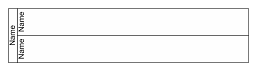
\includegraphics{pic/line.png}\end{center}
\begin{center}
\includegraphics{pic/typs.png}\end{center}

\subsection{Connecting Objects }
\begin{center}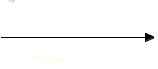
\includegraphics{pic/seqflow.png}\end{center}
\begin{center}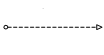
\includegraphics{pic/msgflow.png}\end{center}
\begin{center}
\includegraphics{pic/association.png}\end{center}


\section{Unified Modeling Language}

\section{BPEL???}

\section{SOA???}